\chapter{Présentation du projet}

\section{Contexte et enjeux}
Depuis sa création en 2016, l'entreprise Engie (anciennement GDF-Suez) s'est fortement orientée vers les métiers de la transitions énergétiques. Au travers de sa filiale Engie Green qui détient les actifs éoliens et solaires, elle est devenue en France le leader dans la production d'énergie éolienne avec 1900 MW de capacité installée et leader de la production d'énergie solaire avec une capacité avoisinant les 1200 mégawatt-crêtes (soit un million de watts-crête,  le watt-crête étant l'unité de mesure de la puissance des panneaux photovoltaïques, correspondant à la production de un watt d'électricité).

\begin{figure}[!ht]
\begin{center} \includegraphics[scale=0.5]{rapport/images/Ch1_infog_engiegreen_2017.jpg} \end{center}
\caption{Infographie Engie 2018}
\end{figure}

Le projet fil rouge s'inscrit dans le cadre du projet Engie Darwin, qui consiste à connecter 100\% des unités de productions éoliennes et solaires afin de proposer des nouvelles solutions numériques et maximiser la valeur des installations. Pour les équipes de data scientists du projet, il s'agit de mettre à disposition des exploitants des informations valorisées en temps réel sur le parc de production. L'objectif étant notamment d'anticiper les problèmes de maintenance et d'adapter la production à la demande.

\section{Données à notre disposition}
Ce projet fil rouge de data science concerne plus précisément les données issues de la ferme solaire de Blond en Haute-Vienne (Nouvelle-Aquitaine).

\begin{figure}[!ht]
\begin{center}
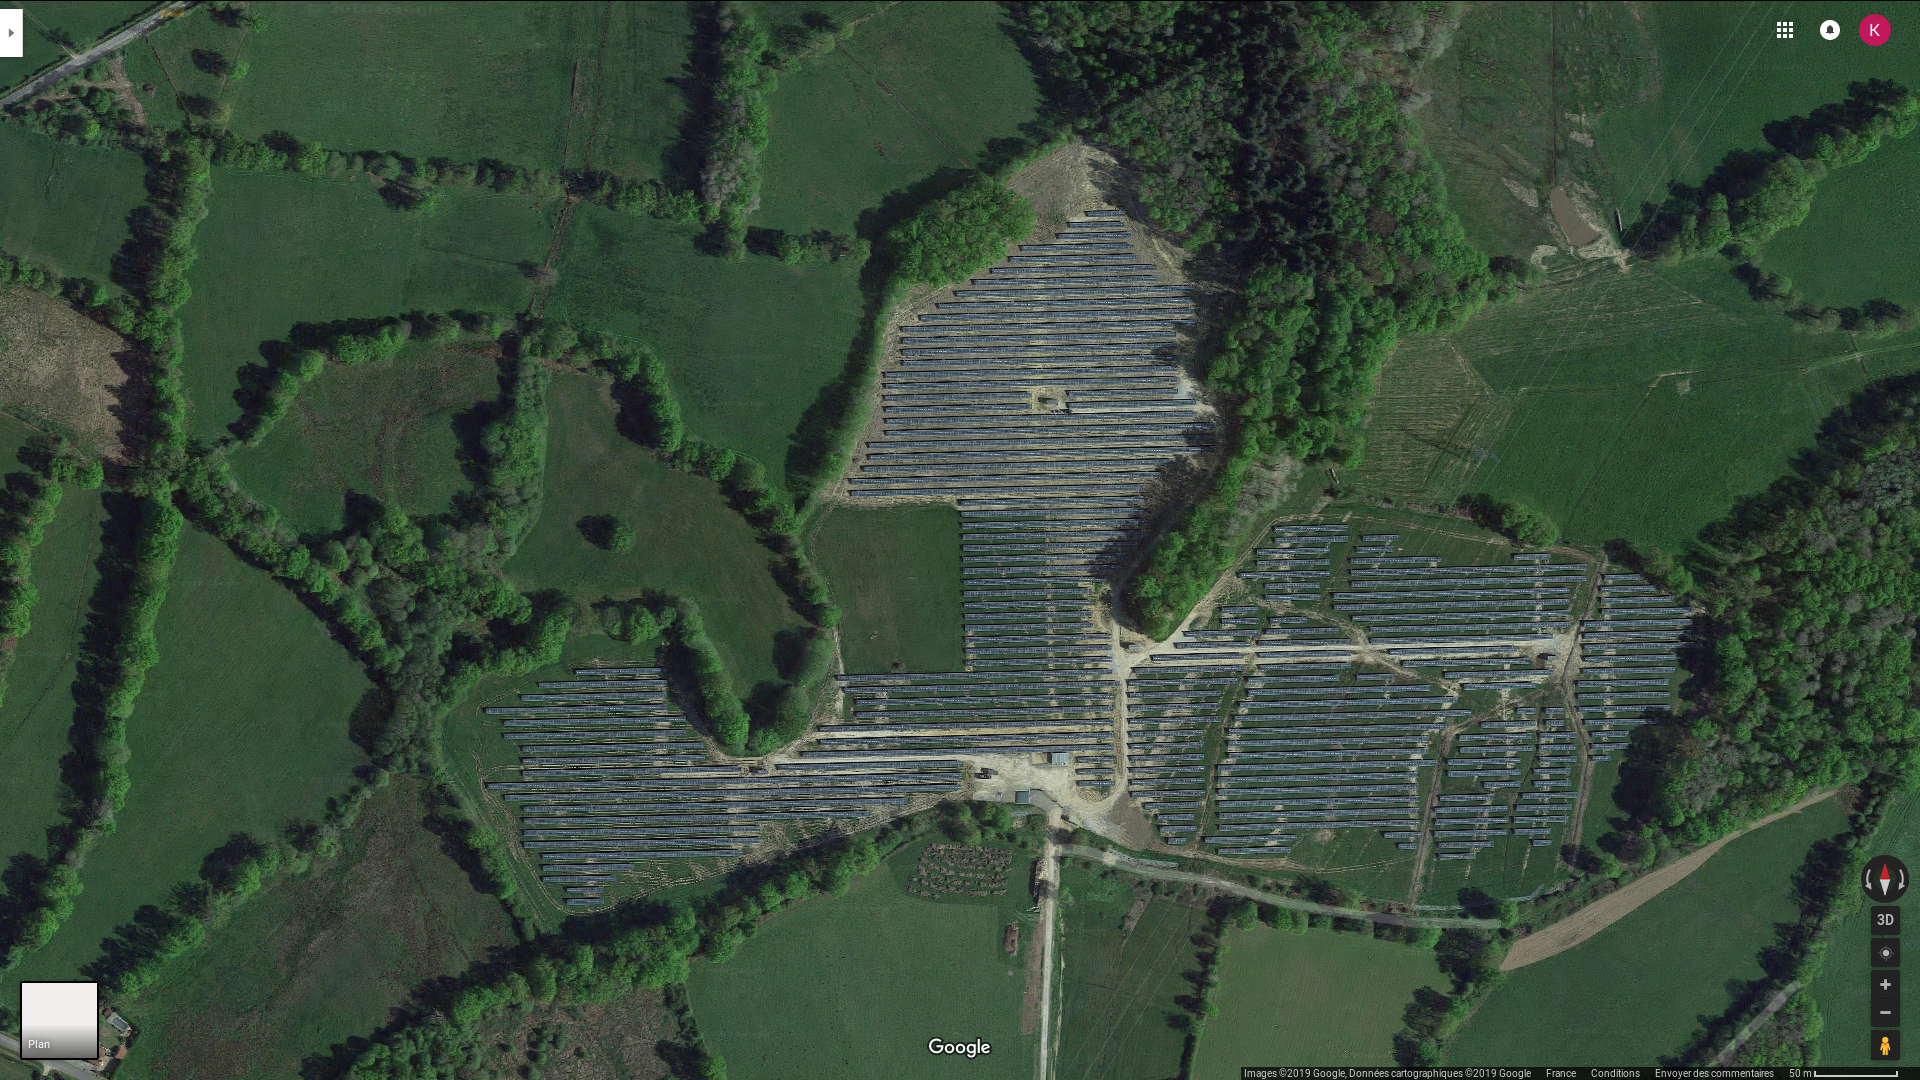
\includegraphics[scale=0.15]{rapport/images/Ch1_FermeSolaire.png}
\end{center}
\caption{La ferme solaire de Blond}
\end{figure}
\FloatBarrier

Cette installation compte près de 25 000 panneaux photo-voltaïques dont le courant électrique produit est agrégé dans des array box, puis des onduleurs avant d'être transformé pour rejoindre le réseau de distribution.

\begin{figure}[!ht]
\begin{center}
\includegraphics[scale=0.4]{rapport/images/Ch1_Onduleurs.png}
\end{center}
\caption{Schéma de l'installation et des onduleurs}
\end{figure}
\FloatBarrier

Les données mises à notre disposition sont de natures différentes :
\begin{itemize}
\item \textbf{Des données de production électrique} en provenance des 8 onduleurs de la ferme, au pas de temps minute. Ces données brutes sont également accompagnées de données prédites issues de 2 modèles réalisés par l'équipe de Paul Poncet.
\item \textbf{Des données météorologiques} mesurées par une station indépendante et comprenant l'irradiance, température, pluviométrie, hygrométrie et vitesse du vent.
\item \textbf{Des données de maintenance} des équipements sous la forme de journal des événements et des interventions sur la ferme.
\end{itemize}
\paragraph{}
\paragraph{}
\paragraph{}
\section{Problématique et objectifs}
À partir des données précédentes, et en particulier des signaux électriques en provenance des panneaux solaires, il s’agit de \textbf{détecter les sous-performances des équipements en analysant les empreintes des différentes perturbations}.  Les "perturbations" ne sont pas nécessairement des anomalies, mais reflètent des facteurs impactant la production, parmi lesquels on peut citer :

\begin{itemize}
\item \textbf{Les effets saisonniers} : la pousse de la végétation par exemple
\item \textbf{Les ombrages} : ombres portées des lignes montagneuses, la végétation, des ouvrages alentours, etc.
\item \textbf{Les déconnexion d’équipements} : ce sont des pertes de lignes ou de strings qui constituent une réelle anomalie de fonctionnement.
\item \textbf{La température des panneaux} : plus la température est élevée, plus l'efficacité des panneaux diminue.
\item \textbf{Les tendances lentes} : la dégradation progressive liée à la perte de rendement des panneaux, par exemple.
\item \textbf{Les salissures / encrassements} : en particulier dans certains pays avec du sable ou de la poussière où les sites sont exposés aux vents. Dans ce cas l'encrassement tend à croître régulièrement jusqu'à ce qu'une forte averse de pluie vienne nettoyer les panneaux. \cite{JavedW}
\end{itemize}

\begin{figure}[!ht]
\begin{center}
\includegraphics[scale=0.8]{rapport/images/Ch1_SchemaEncrassement.png}
\end{center}
\caption{Schéma du phénomène d'encrassement}
\end{figure}
\FloatBarrier

Dans un contexte de production, l'information de ces sous-performance et la détection des anomalies avérées seraient transmises à l’exploitant pour action.

\section{Approche proposée par Engie}
Outre nos recherches bibliographiques, deux approches nous ont été suggérées pour traiter le problème :
\begin{enumerate}
\item \textbf{Une approche globale} visant à retrouver les effets de façon simultanée et à définir ce que serait le signal normal.
\item  \textbf{Une approche par décomposition du signal par onduleur}, basée les résidus issus de la différence entre les données brutes et les modèles créés par Engie. L'utilisation d'une décomposition par ondelettes a été suggérée pour retrouver les signatures typiques du signal.
\end{enumerate}
%\let\clearpage\relax